\section{Modéliser et approcher}

\begin{frame}{Le modèle : affecter chaque patient à une vacation}
  \scriptsize
  \begin{columns}[T,onlytextwidth]
    \begin{column}{0.46\textwidth}
      \begin{block}{Décision}
        \[
          x_{i,v}\in\{0,1\},\qquad
          \sum_{v\in V_i}x_{i,v}=1
        \]
        \begin{tabular}{@{}ll@{}}
          $x_{i,v}$ & patient $i$ affecté à la vacation $v$ \\
          $V_i$ & vacations compatibles \\
          $d_i$ & durée opératoire estimée \\
        \end{tabular}
      \end{block}

      \uncover<2->{%
      \begin{block}{Contraintes dures}
        \begin{itemize}
          \item une vacation par patient ;
          \item capacité de vacation non dépassée ;
          \item capacité de lits respectée chaque jour ;
          \item fenêtre clinique des urgences respectée.
        \end{itemize}
      \end{block}}
    \end{column}

    \begin{column}{0.52\textwidth}
      \begin{alertblock}{Objectif}
        \[
          \min\; \alpha\,\Delta_{\text{vac}}
          +\beta\,\Delta_{\text{lits}}
          +\gamma\,\sigma_{\text{vac}}
        \]
        \[
          \alpha=5{,}0,\qquad \beta=3{,}0,\qquad \gamma=0{,}05
        \]
        \begin{itemize}
          \item $\Delta_{\text{vac}}$ : minutes au-delà des vacations ;
          \item $\Delta_{\text{lits}}$ : dépassement de capacité en lits ;
          \item $\sigma_{\text{vac}}$ : écart-type de charge des vacations.
        \end{itemize}
      \end{alertblock}
    \end{column}
  \end{columns}
\end{frame}

\begin{frame}{Pipeline ML}
  \scriptsize
  \begin{columns}[T,onlytextwidth]
    \begin{column}{0.47\textwidth}
      \centering
      \begin{tikzpicture}[
        n/.style={draw=McmTerracotta,rounded corners=3pt,fill=white,
                  text width=4.1cm,minimum height=0.75cm,align=center,
                  font=\scriptsize,inner sep=2pt},
        f/.style={-{Latex[length=2mm]},thick,draw=McmTerracotta}]
        \node[n] (a) at (0,0) {\textbf{Données brutes}\\14\,434 cas, 30 colonnes};
        \node[n] (b) at (0,-1.15) {\textbf{Nettoyage}\\73 exclusions, séjour corrigé};
        \node[n] (c) at (0,-2.30) {\textbf{Split temporel par patient}\\2019--2021 $\rightarrow$ 2022};
        \node[n] (d) at (0,-3.45) {\textbf{Trois cibles}\\salle, séjour, ambulatoire};
        \draw[f] (a) -- (b);
        \draw[f] (b) -- (c);
        \draw[f] (c) -- (d);
      \end{tikzpicture}
    \end{column}

    \begin{column}{0.51\textwidth}
      \begin{alertblock}{Les pièges traités}
        \begin{itemize}
          \item valeurs manquantes explicites, sans imputation inventée ;
          \item heures nulles exclues, pas imputées ;
          \item aucune fuite : dates, durées et identifiants exclus.
        \end{itemize}
      \end{alertblock}

      \uncover<2->{\par\vspace{0.12cm}\footnotesize \textbf{Sorties :} durée en salle,
        durée de séjour, ambulatoire}
    \end{column}
  \end{columns}
  \source{Notebooks de prétraitement du dépôt.}
\end{frame}

\begin{frame}{Trois métaheuristiques}
  \footnotesize
  NP-difficile : on cherche une bonne solution en temps borné, avec la même
  interface pour toutes les méthodes.

  \vspace{0.15cm}
  \renewcommand{\arraystretch}{1.18}
  \begin{tabular}{p{2.9cm}p{4.5cm}p{4.5cm}}
    \toprule
    \textbf{Méthode} & \textbf{Principe} & \textbf{Effet} \\
    \midrule
    Recuit simulé & Explorer largement, accepter de remonter
      & Évite les optima locaux \\
    Recherche Tabou & Intensifier le meilleur voisin non tabou
      & Mémoire des mouvements, évite le cyclage \\
    Algorithme génétique & Croiser une population de solutions
      & Diversité ; recombine de bonnes parties \\
    \bottomrule
  \end{tabular}

  \uncover<2->{\par\vspace{0.18cm}\footnotesize Les hybrides enchaînent une
    exploration globale et une intensification locale.}
  \source{Formulation du projet ; revues Amin et al. (2024) et Rachuba et
    al. (2024).}
\end{frame}

\begin{frame}{Solution proposé : Hybrides}
  \footnotesize
  \begin{columns}[T,onlytextwidth]
    \begin{column}{0.54\textwidth}
      \begin{block}{Quatre hybrides}
        \begin{itemize}
          \item \textbf{Tabou $\times$ Recuit} : voisinage tabou et acceptation
            de Metropolis.
          \item \textbf{Génétique $\times$ Tabou} : tabou courte sur le meilleur
            individu.
          \item \textbf{Génétique $\times$ Recuit} : recuit courte sur le
            meilleur individu.
          \item \textbf{Fourmis $\times$ Tabou} : intensification de la
            meilleure fourmi.
        \end{itemize}
      \end{block}
    \end{column}

    \begin{column}{0.44\textwidth}
      \footnotesize
      Une méthode globale explore ; une méthode locale intensifie.

      \uncover<2->{\par\vspace{0.12cm}Génétique $\times$ Tabou divise l'écart
        du génétique par $\sim$$10^4$ ; Fourmis $\times$ Tabou divise l'écart
        ACO par $\sim$1,7.}
    \end{column}
  \end{columns}
  \source{Distinct de l'hybride d'origine Tabou $\times$ Recuit ; les trois
    autres hybrides ont été construits pour ce projet.}
\end{frame}

\begin{frame}{Validation exacte, puis changement d'échelle}
  \small
  \begin{columns}[T,onlytextwidth]
    \begin{column}{0.48\textwidth}
      \begin{exampleblock}{Petite instance}
        \footnotesize 7 patients, 4 vacations, $4^7=16\,384$ combinaisons.
        Les 10 méthodes atteignent l'optimum sur 20 graines.
      \end{exampleblock}
      \centering
      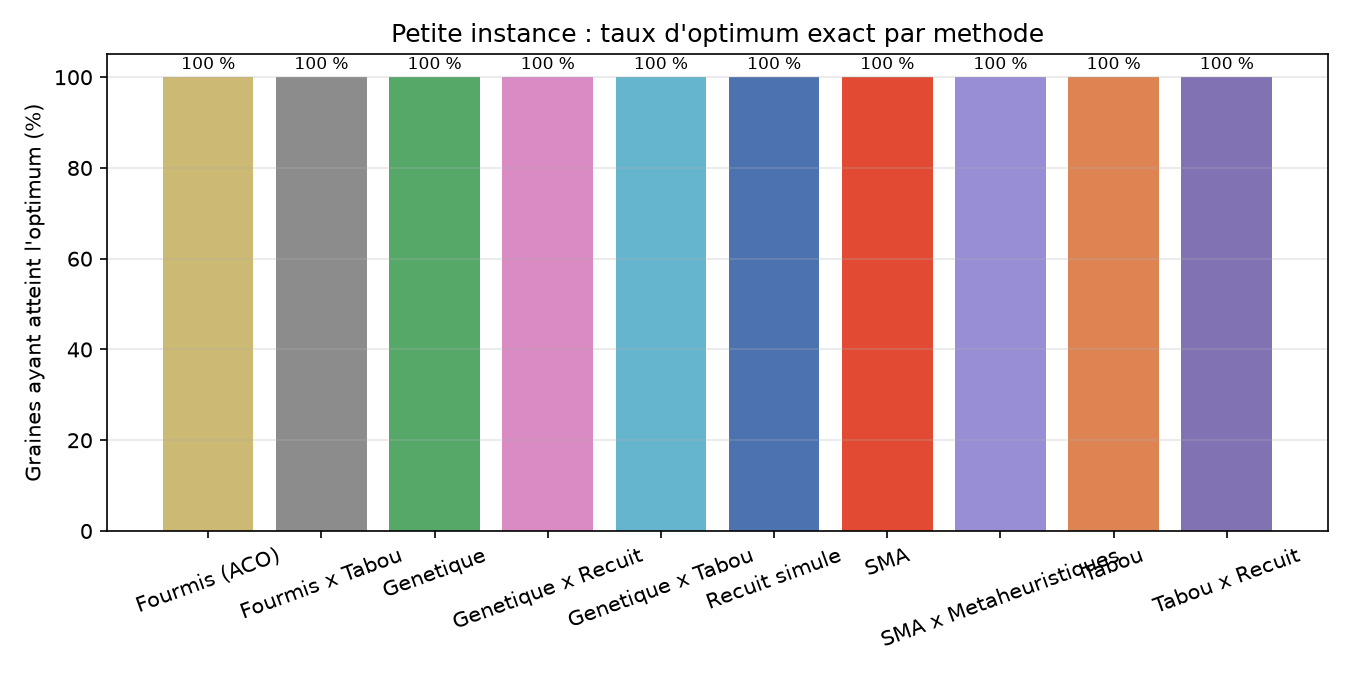
\includegraphics[width=0.95\linewidth,height=0.38\textheight,keepaspectratio]{petite_taux_optimum.png}
      \credit{10/10 méthodes à l'optimum exact.}
    \end{column}

    \begin{column}{0.50\textwidth}
      \centering
      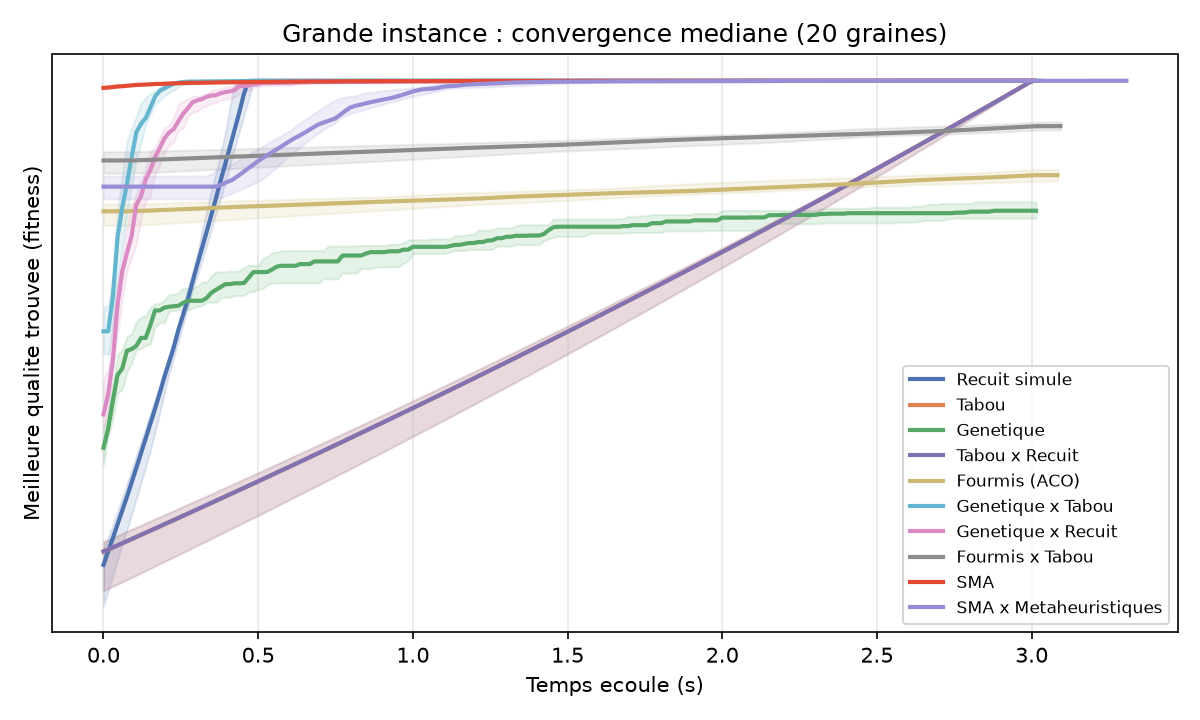
\includegraphics[width=\linewidth,height=0.44\textheight,keepaspectratio]{grande_convergence.png}
      \credit{Convergence médiane, 300 patients, 3 s, 20 graines.}
      \uncover<2->{\par\vspace{0.12cm}\footnotesize Le planning est optimal
        pour les durées prévues. Une urgence,\textbf{ une annulation ou une salle
        fermée suffit à le rendre inadapté.}}
    \end{column}
  \end{columns}
\end{frame}

\begin{frame}{Aléas : les quatre cas principaux}
  \scriptsize
  \begin{block}{Quatre aléas principaux}
    \begin{itemize}
      \item \textbf{Urgence} : patient imprévu, fenêtre temporelle imposée ;
        à insérer dans une vacation compatible.
      \item \textbf{Annulation} : patient programmé qui annule ; libère un
        créneau \textbf{et} des lits.
      \item \textbf{Indisponibilité de lits} : capacité réduite sur un
        intervalle ; réaffecter les séjours chevauchants.
      \item \textbf{Retard bloc} : prolongation ou incident sur une
        vacation ; capacité utile réduite.
    \end{itemize}
  \end{block}

  \par\vspace{0.04cm}
  {\footnotesize \textbf{HAS 2026} : environ 10\,\% des interventions
    programmées sont annulées, la plupart reprogrammées.}

  \uncover<2->{%
  \par\vspace{0.10cm}
  \begin{columns}[T,onlytextwidth]
    \begin{column}{0.46\textwidth}
      \begin{block}{Statique}
        \footnotesize Un plan nominal, optimisé pour les durées prévues.
        C'est la référence de départ.
      \end{block}
    \end{column}
    \begin{column}{0.52\textwidth}
      \begin{exampleblock}{Dynamique}
        \footnotesize Le plan est maintenu dans le temps : dates de repli
        proactives, puis replanification réactive.
      \end{exampleblock}
    \end{column}
  \end{columns}}
  \source{Chaque aléa a sa classe et son simulateur reproductible
    (\texttt{generer\_scenario\_aleas}).}
\end{frame}

\begin{frame}{Dynamique : préparer des dates de substitution}
  \scriptsize
  \begin{columns}[T,onlytextwidth]
    \begin{column}{0.46\textwidth}
      \begin{block}{Quatre profils de repli}
        \begin{itemize}
          \item \textbf{Nominal} : planning optimal à 100\,\% de la capacité.
          \item \textbf{Robuste avec marge} : 15\,\% de capacité laissée libre
            (bloc + lits) pour absorber un aléa sans déplacer les patients.
          \item \textbf{Sécurité lits} : lissage strict, sous-saturation
            volontaire.
          \item \textbf{Date B} : bonne qualité, différente du nominal.
        \end{itemize}
      \end{block}
    \end{column}

    \begin{column}{0.52\textwidth}
      \footnotesize Une Date A optimale, une Date B alternative, avec leurs
      raisons.

      \par\vspace{0.12cm}
      \renewcommand{\arraystretch}{1.25}
      \centering
      \begin{tabular}{@{}p{1.9cm}p{1.45cm}p{1.45cm}p{1.75cm}@{}}
        \toprule
        Patient & Date A & Date B & Arbitrage \\
        \midrule
        Mme D. & 12 mars & 26 mars & lits tendus \\
        M. K. & 14 mars & 21 mars & bloc saturé \\
        Mme R. & 15 mars & 18 mars & équipe \\
        \bottomrule
      \end{tabular}

      \uncover<2->{\par\vspace{0.12cm}Le chirurgien voit la date, l'occupation
        du bloc et des lits, et la raison de l'écart.}
    \end{column}
  \end{columns}
  \source{Extraction : \texttt{extraire\_options\_date\_a\_b}.}
\end{frame}

\begin{frame}{Dynamique / réactif : replanifier sans tout déplacer}
  \scriptsize
  \begin{columns}[T,onlytextwidth]
    \begin{column}{0.53\textwidth}
      \begin{block}{Trois garde-fous}
        \begin{itemize}
          \item \textbf{Gel du passé} : actes commencés ou programmés
            sanctuarisés.
          \item \textbf{Urgences} : insertion prioritaire dans la fenêtre
            clinique.
          \item \textbf{Moindre perturbation} : limiter déplacements et
            changements de jour.
        \end{itemize}
      \end{block}

      \uncover<2->{%
      \begin{alertblock}{Score d'adaptation}
        \[
          \begin{aligned}
            \text{Score} = \text{Fitness}
            &- w_p \cdot \text{déplacements}\\
            &- w_j \cdot \text{changements de jour}
          \end{aligned}
        \]
        Le planning reste proche de celui annoncé aux patients.
      \end{alertblock}}
    \end{column}

    \begin{column}{0.45\textwidth}
      \centering
      \begin{tikzpicture}[
        ag/.style={draw=McmSage,rounded corners=2pt,fill=McmSage!10,
                   minimum height=0.55cm,minimum width=1.55cm,align=center,
                   font=\tiny},
        bb/.style={draw=McmTerracotta,rounded corners=2pt,
                   fill=McmTerracotta!10,minimum height=1.95cm,
                   minimum width=1.85cm,align=center,font=\tiny,thick},
        co/.style={draw=McmAmber,rounded corners=2pt,fill=McmAmber!10,
                   minimum height=0.5cm,minimum width=1.85cm,align=center,
                   font=\tiny},
        f/.style={-{Latex[length=1.7mm]},thick,draw=McmTerracotta}]
        \node[ag] (a1) at (0,0) {Agent recuit};
        \node[ag] (a2) at (0,-0.85) {Agent tabou};
        \node[ag] (a3) at (0,-1.70) {Agent génétique};
        \node[bb] (bb) at (2.55,-0.85) {\textbf{Tableau noir}\\meilleure\\solution};
        \node[co] (co) at (2.55,0.55) {\textbf{Coordinateur}};
        \draw[f] (a1.east) -- (bb.west|-a1);
        \draw[f] (a2) -- (bb);
        \draw[f] (a3.east) -- (bb.west|-a3);
        \draw[f,draw=McmAmber] (co) -- (bb);
      \end{tikzpicture}
      \uncover<2->{\par\vspace{0.10cm}\footnotesize Agents par cycles
        courts, versionnement de la meilleure solution, migration si
        stagnation.}
    \end{column}
  \end{columns}
  \source{Implémentation Mesa 3.5 : agents simples et agents
    métaheuristiques coopérant par tableau noir.}
\end{frame}

\againframe<4>{recap}
